% v2-acmtog-sample.tex, dated March 7 2012
% This is a sample file for ACM Transactions on Graphics
%
% Compilation using 'acmtog.cls' - version 1.2 (March 2012), Aptara Inc.
% (c) 2010 Association for Computing Machinery (ACM)
%
% Questions/Suggestions/Feedback should be addressed to => "acmtexsupport@aptaracorp.com".
% Users can also go through the FAQs available on the journal's submission webpage.
%
% Steps to compile: latex, bibtex, latex latex
%
% For tracking purposes => this is v1.2 - March 2012
\documentclass{acmtog} % V1.2

%\acmVolume{VV}
%\acmNumber{N}
%\acmYear{YYYY}
%\acmMonth{Month}
%\acmArticleNum{XXX}
%\acmdoi{10.1145/XXXXXXX.YYYYYYY}
\acmVolume{28}
\acmNumber{4}
\acmYear{2019}
\acmMonth{September}
\acmArticleNum{106}
\acmdoi{10.1145/1559755.1559763}

\usepackage{booktabs}

\begin{document}

% \markboth{Recommendation Algorithm}{Collaborative Filtering Algorithm Optimization}

\title{User Influence Analysis by Ripple Network on micro-blog Social Networks } % title

\author{Shengyuan Huang {\upshape and} Buqing Nie
\affil{Shanghai Jiao Tong University}
% NOTE! Affiliations placed here should be for the institution where the
%       BULK of the research was done. If the author has gone to a new
%       institution, before publication, the (above) affiliation should NOT be changed.
%       The authors 'current' address may be given in the "Author's addresses:" block (below).
%       So for example, Mr. Fogarty, the bulk of the research was done at UIUC, and he is
%       currently affiliated with NASA.
}


\maketitle
% \section*{Abstract}


\section{Introduction}

%%%%%  模型图
\begin{figure*}
\centering
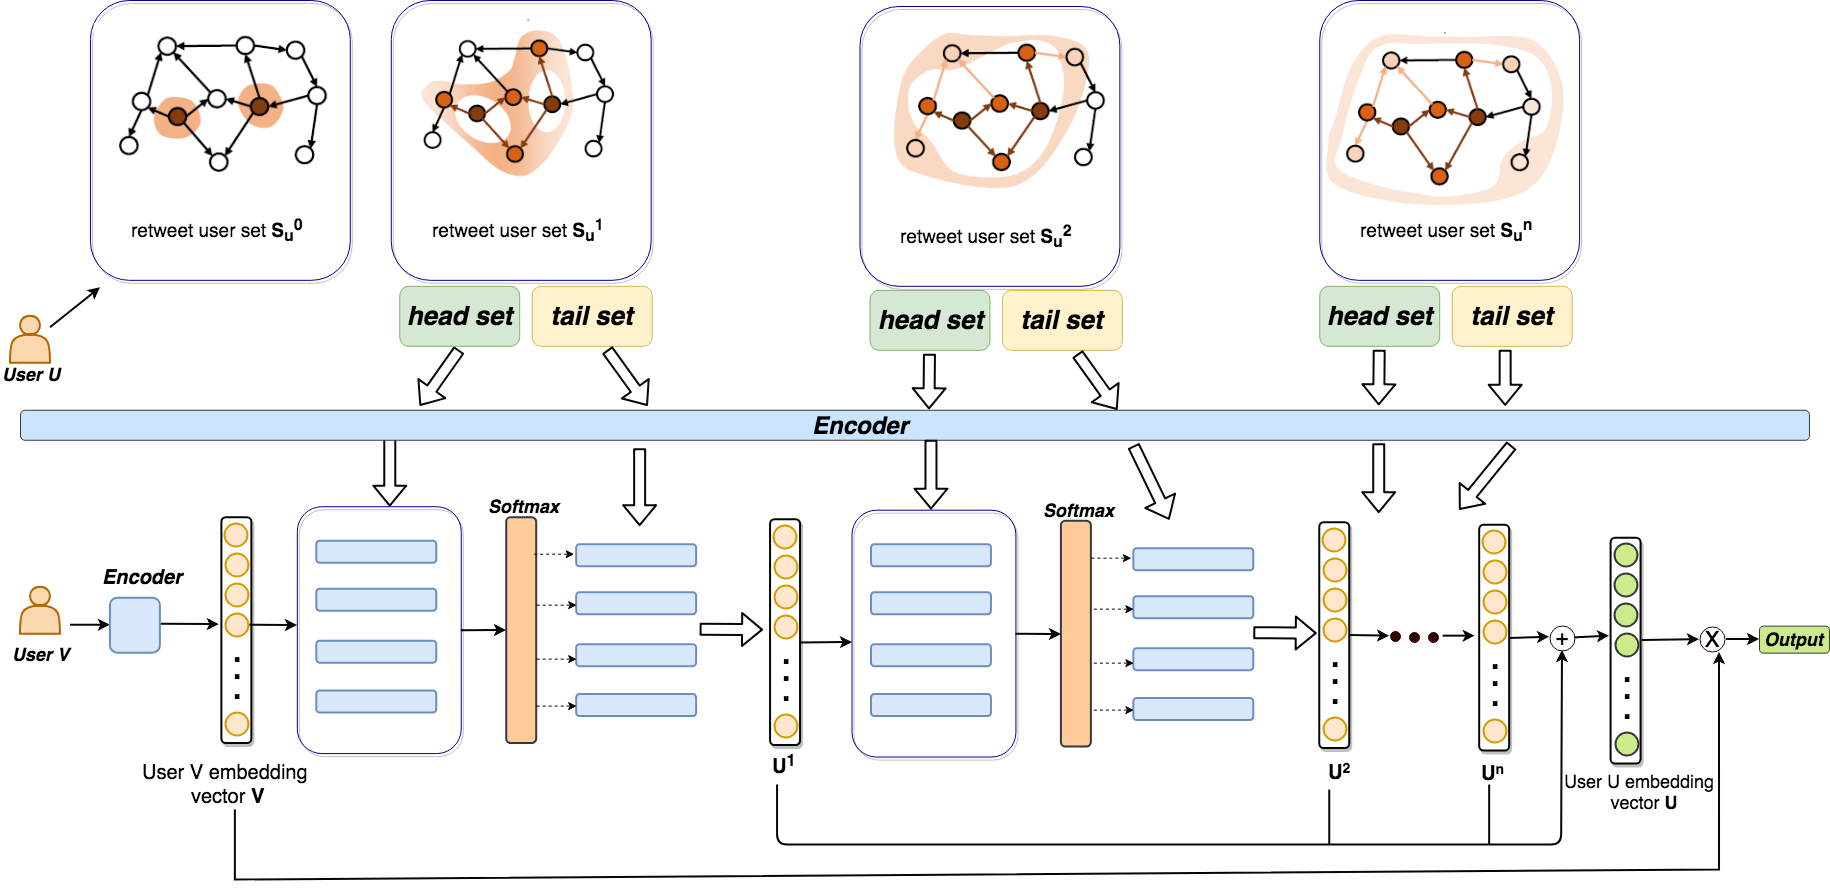
\includegraphics[width=14cm]{model.png}
\caption{The overall framework of our model. It takes a user $u$ and a user $v$ as input, and outputs the predicted user $v$'s influence to user $u$.}
\end{figure*}

\subsection{Background}
Recently, the micro-blog plays more and more important role in our daily life, which has become a main approach to receiving information from the network. However, the number of users on social network like twitter, micro-blog has risen sharply. Meanwhile, the amount of information on social media is exploding everyday. There are more and more information of low quality, which are difficult for us to distinguish.

Moreover, The experiment tell us in each social media, there are some influential users who can predetermine the topics for discussion and the attitudes to certain events or persons to a large extent. And we can seen these influential users as good information sources. 

Besides, many commercial agents such as many advertising company need to identify opinion leaders and maximize the dissemination of the advertise message by analyzing existing micro-blogs. Thus, they need to compute the user influence value through analyzing the micro-blog logs.

In addition, the user influence estimation could be applied for friends recommendation, information dissemination prediction, user behavior prediction, etc. Above all, the user influence estimation has become an important aspect of
informational and analytic work with social networks, which is the main problem we want to solve in this project.

\subsection{Motivation}

In this project, we want to transfer Ripple Network\cite{wang2018ripple} model from Recommend systems to the user influence estimation in the social network, expecting a good performance compared to the existing models.

For any user $u$, we can estimate the influence value of $u$ in the given social network, then we can believe that user $u$ is a high quality information source, and the blogs he/she posted are information of high quality. The probability that the other users retweet his/her blogs is higher than other users.

\subsection{contributions}
The main contributions of this project can be summarized in these points:
\begin{enumerate}
    \item We transfer Ripple Network model from Recommend systems to the user influence estimation in the social network to estimate the user influence value.
    \item We start an experiment to show the performance of the Ripple Network in the user influence estimation region.
\end{enumerate}


\section{Related Work}
The user influence is one of the hot topics in the social network because of its wide application. The followings are the state-of-the-art related works in the recent years.

\subsection{Ripple Network}

The Ripple Network is an end-to end framework that naturally incorporates the knowledge graph into recommender systems for knowledge-graph-aware
recommendation.The key idea behind Ripple Network is preference propagation: For each user, Ripple Network treats his historical interests as a seed set in the KG, then extends the user’s interests iteratively
along KG links to discover his hierarchical potential interests with
respect to a candidate item.\cite{wang2018ripple}

\subsection{User influence estimation}

\subsubsection{Rank-based model}
Rank-based model usually measures users’ influence by exploiting the link relationship between the users with an iterative algorithm. They are mainly based on the Page Rank algorithm, like PageRank based model TwitterRank\cite{weng2010twitterrank} which measures posters’ influence by taking into account the link structure of followers/following of individual users and the topical similarity between these users.Li et al. \cite{li2011casino} proposed an iterative algorithm to calculate the influence of the individual in the social network by conformity. The conformity in his model is defined as the probability that an individual is willing to accept others’ opinions.

\subsubsection{Feature-based model}
Feature-based model measures users’ influence by exploiting the social features in specific media like the number of followers and posts in the context of twitter. In the context of twitter, Pal and Counts\cite{ou2016asymmetric} proposed a model Twitter Authority that uses the count of original tweets, conversational tweets, and retweets of a tweeter as features to rank the authority of each tweeter in different topics.In the context of blog, Agarwal et al. \cite{agarwal2008identifying} proposed a model to measure the influence of bloggers. They think of bloggers posted enough influential blogs as influential bloggers.

\subsection{Network Embedding}
Network embedding methods aim at learning low-dimensional latent representation of nodes in a network, which has become a popular method to manipulate the network data. The network embedding can be categorized into Random Walk based methods, Edge modeling based methods, and Matrix factorization based methods.

The random walk based methods implement the function by performing truncated random walks. The information network is transformed into a collection of vertex sequences, in which, the occurrence frequency of a vertex-context pair measures the structural distance between them. The most popular one is DEEPWALK\cite{perozzi2014deepwalk}.

Edge modeling based methods directly learn vertex  representations from vertex-vertex connections. One popular method is LINE\cite{tang2015line}.

Matrix factorization based methods represent the connections between network ertices in the form of a matrix and use matrix factorization to obtain the embeddings. One popular method is HOPE\cite{ou2016asymmetric}.

% \begin{figure*}
% \centering
% 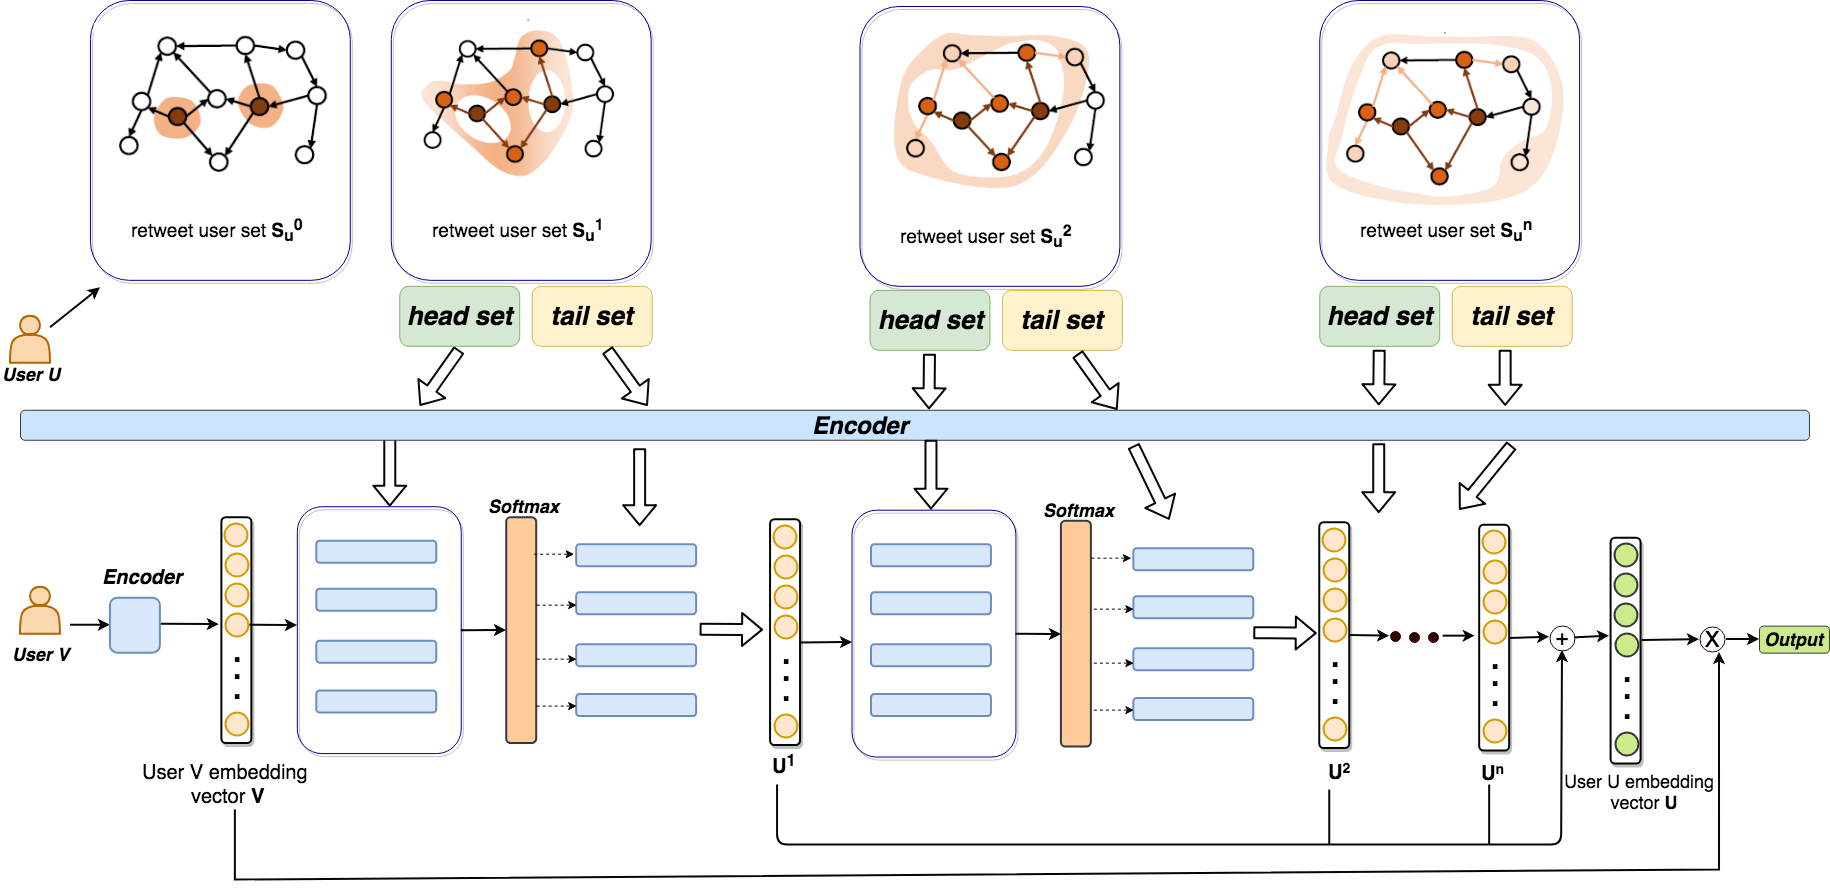
\includegraphics[width=12cm]{model.png}
% \caption{The overall framework of our model. It takes a user $u$ and a user $v$ as input, and outputs the predicted user $v$'s influence to user $u$.}
% \end{figure*}

\section{Proposed Methods}

\subsection{Problem Formulation}

\begin{enumerate}
    \item \emph{user-user influence matrix:} In our project, let $U=\{u_1,u_2 ...\}$ denotes the sets of users. The user-user influence matrix $Y=\{y_{uv}|u,v\in U\}$ is defined according to users' action, where $y_{uv}=1$ if user u read and retweet user v's weibo. 
    
    \item \emph{Social network graph:} $G = (V, E)$ notes a social network. $V$ denotes users,$E$ is the set of relationships between users, which consists of the information of following. That is, if user u follows user v, there is a directed edge from u to v in G. In other words, there are massive directed edge (u',v') in G, where $u'\in U, v'\in U$ denote user u and the user v. The Fig\ref{social network} is an example social network graph.
\end{enumerate} 

\begin{figure}
\centering
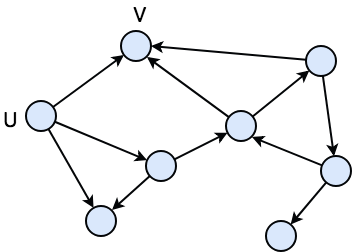
\includegraphics[width=5cm]{network.png}
\caption{One example of the social network graph}
\label{social network}
\end{figure}

Given an influence matrix Y as well as a graph G, we aim to predict user v's influence to user u. Our goal is to learn a prediction function $\hat{y}_{uv}=F(u,v;\theta)$, where $\hat{y}_{uv}$ denotes the user v's influence to user u, and $\theta$ denotes the model parameters of function F.

\subsection{the model of  the problem}

The framework of our model is illustrated in the Figure. It takes a user u and a user v as input, and outputs the predicted user v's influence to user u. We define 
$$S^k_{u}=\{v'|(u',v') \in G \quad and \quad u' \in S^{k-1}_{u} \}, k = 1, 2, ...,n.$$
$$S^0_u=V_u=\{v|y_{uv}=1\}$$
For the input user u, his following set of $V_u$ is treated as seeds in G, then extended to form multiple sets $E^k_u$(k = 1,2,...,n), where 
$$E^k_{u}=\{(u',v')|(u',v') \in G \quad and \quad u' \in S^{k-1}_{u} \}, k = 1, 2, ...,n.$$ 
These sets are used to interact with the user v's embedding for obtaining the responses of user u with respect to user v, which are then combined to form the final user u's embedding. Lastly, we use the embeddings of user u and user v together to compute the predicted user v's influence to user u $\hat{y}_{uv}.$

 Also, as is shown in the Figure, the user v is associated with an embedding $v\in R^d$ through a certain encoder(such as the one-hot encoder), where d is the dimension of embeddings. Given the embedding v and the 1-hop set $E^1_u$ of user u, each tuple $(u'_i,v_i')$ in $E^1_u$ is assigned a relevance probability by comparing v to the $u'_i$ in this tuple:
 $$p_i=softmax(v^T u'_i)=\frac{exp(v^T u'_i)}{\sum_{(u',v')\in E^1_u} exp(v^T u')}$$, where $u'_i \in R^d$  are the embeddings of $u'_i$. After obtaining the relevance probabilities, we take the sum of v' in $E^1_u$ weighted by the corresponding relevance probabilities,
and the vector $U^1$ is returned: $$U^1=\sum_{(u'_i,v'_i)\in E^1_u} p_i v'_i$$, where $v'_i \in R^d$ is the embedding of $v'_i$. Repeating the procedure, we can get $U^1,U^2...U^n$. Then we can get the embedding of user u with respect to user v: 
$$u=\alpha_1 H^1+\alpha_2 H^2+...+\alpha_n H^n$$, where $\alpha_i$s are positive trainable parameters.\\

Finally, the embedding of u and the embedding of v are combined to output the predicted user v's influence to user u:
$$\hat{y}_{uv}=\sigma(u^T v)$$
$$\sigma(x)=\frac{1}{1+exp(-x)}$$.

\section{Experiment}
To verify the performance of the Ripple Network in the social influence estimation, we conduct an user retweet behavior prediction experiment on the Sina micro-blog social network.

In the experiment, if the influence value $v_{uv}$ of user $u$ to user $v$ less than 0.5, we assume that user $v$ won't retweet the micro-blog of user $u$. Otherwise, he will reweet the micro-blog.

\subsection{Dataset}
The dataset used in our eperiment is the Sina micro-blog public data on the \emph{aminer.cn}, which is a quite big dataset, the following are the introduction of the datset:

\begin{table}[htp]
\centering
\begin{tabular}{|c|c|}
 \hline
 Dataset Source &Sina micro-blog \\
 \hline
\#Users & 1,776,950  \\
 \hline
\#Follow relationships & 308,489,739  \\
 \hline
\#Original micro-blogs & 300,000 \\
\hline
\#Retweets & 23,755,810 \\
 \hline
\end{tabular}
\end{table}

Because the dataset is too big for us to conduct he experiment, so the dataset used in our experiment is simplified. 

% \subsection{Baselines}

% \begin{enumerate}
%     \item 
% \end{enumerate}

\subsection{Results}
The Fig\ref{fig:result01} shows that the convergence is very quickly, however, the result of the test dataset is not satisfactory. The Fig\ref{fig:redis} is the influence value distribution figure on our dataset, the distribution is quite smooth, which is expected.

The Fig7 is the comparasion between the Ripple Network and other existing models.

\begin{figure}
    \centering
    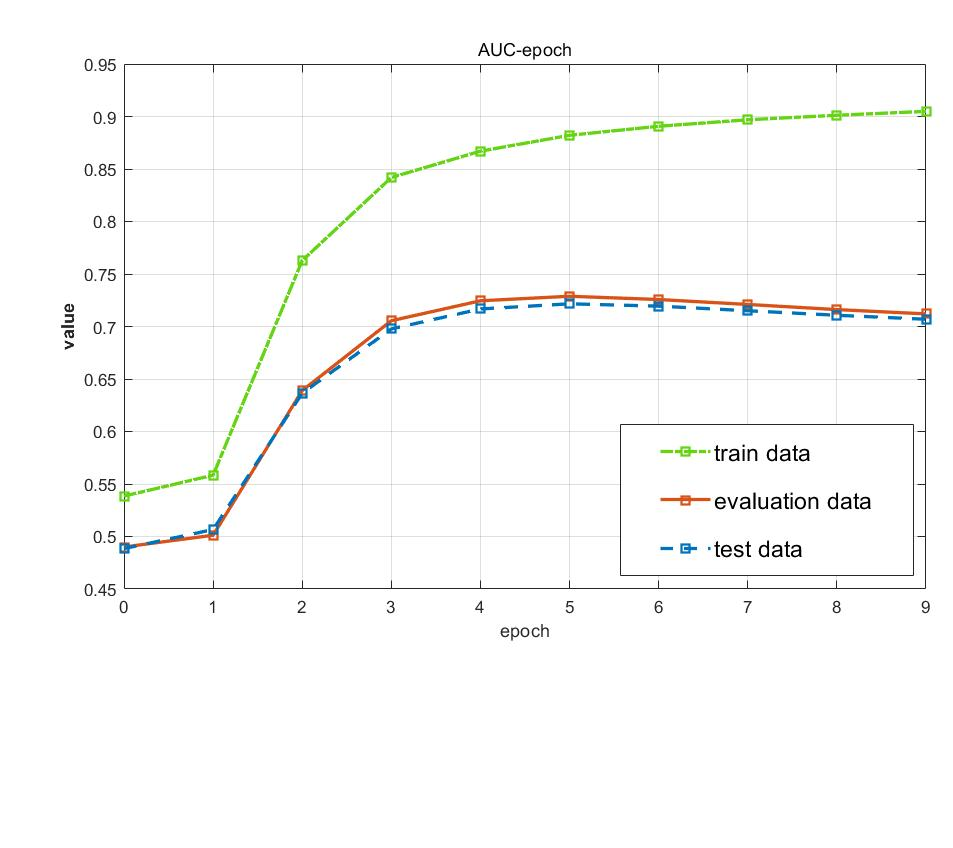
\includegraphics[width=4cm]{auc_epoch.jpg}
    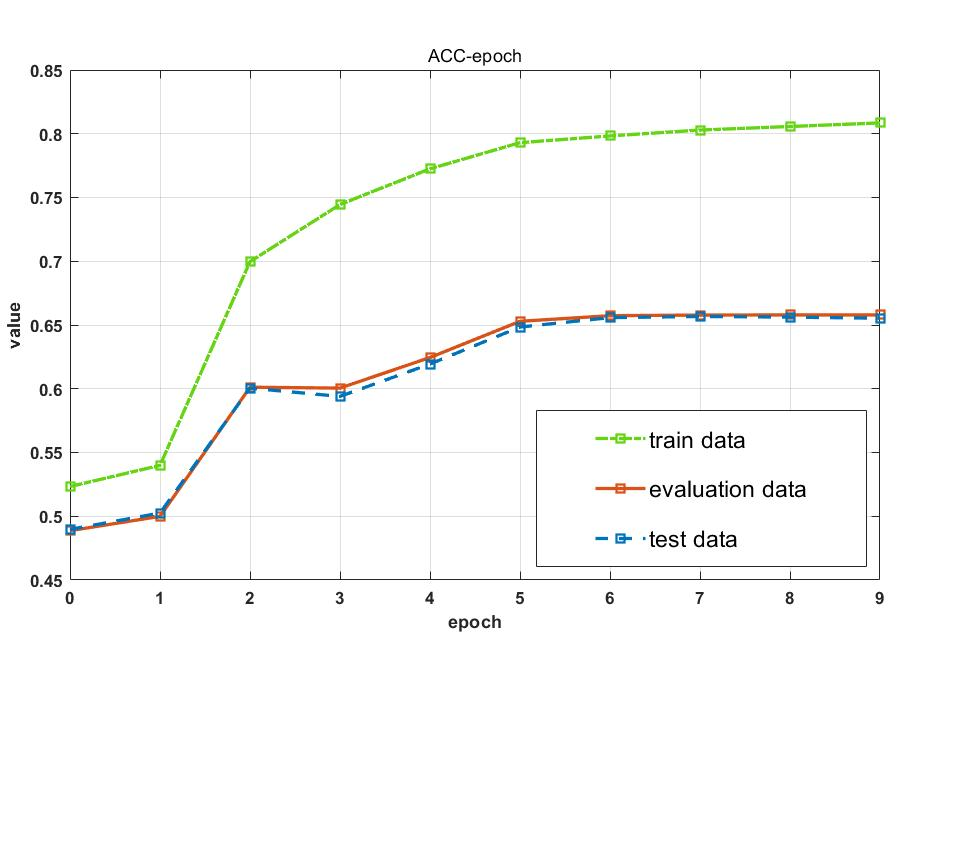
\includegraphics[width=4cm]{acc_epoch.jpg}
    \caption{The AUC and accuracy - epoch result}
    \label{fig:result01}
\end{figure}

\begin{figure}
    \centering
    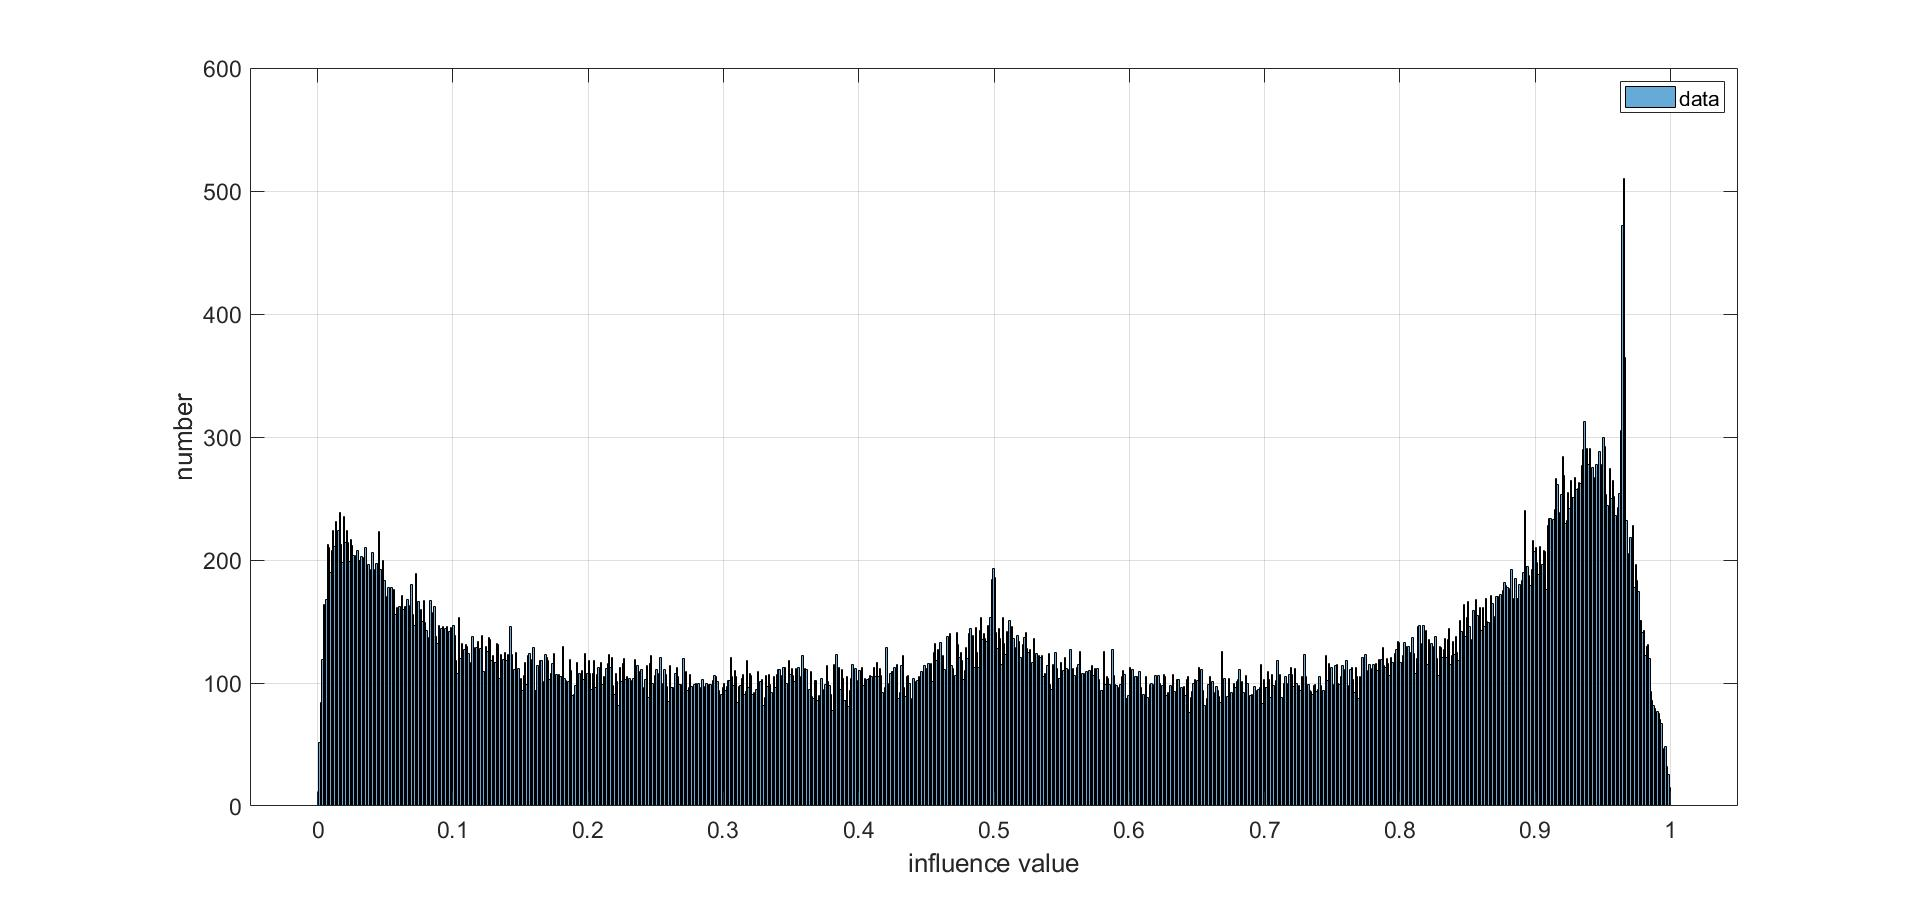
\includegraphics[width=8cm]{re_dis.jpg}
    \caption{The influence value distribution in our dataset}
    \label{fig:redis}
\end{figure}


\section{Discussion}

\begin{figure}
    \centering
    \includegraphics{}
    \caption{Caption}
    \label{fig:my_label}
\end{figure}

\begin{figure}
    \centering
    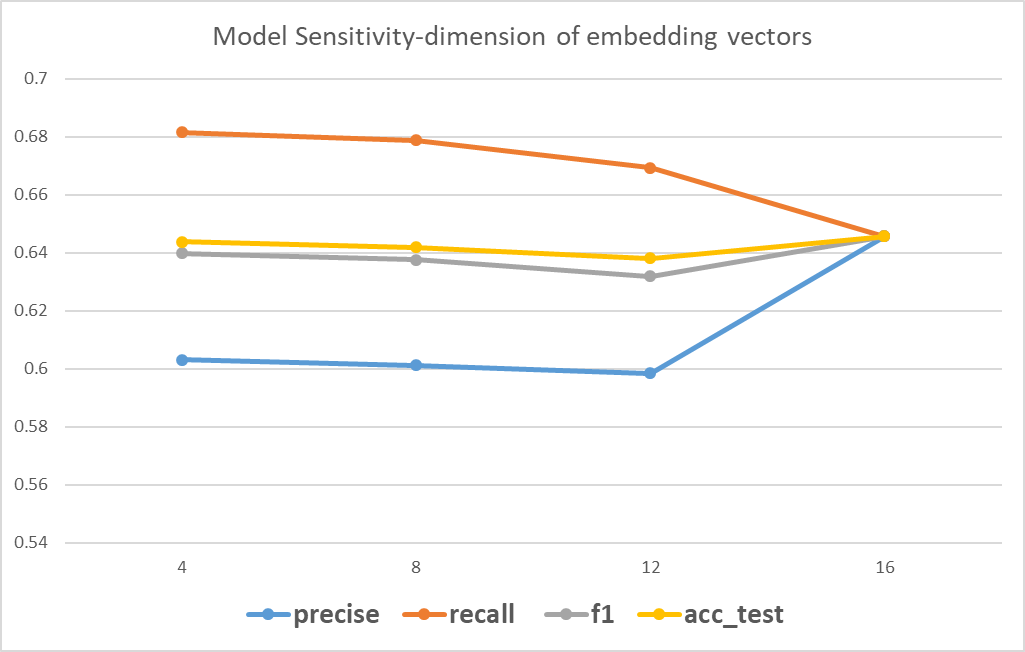
\includegraphics[width=8cm]{sen.png}
    \caption{Model sensitivity analysis}
    \label{fig:sen}
\end{figure}

\begin{figure}
    \centering
    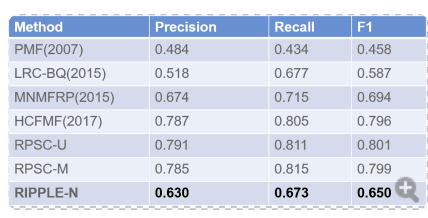
\includegraphics[width=8cm]{re.png}
    \caption{Model sensitivity analysis}
    \label{fig:sen}
\end{figure}

The Fig5\ref{fig:sen} is the precision-$d$ figure, $d$ is the dimension of embedding vectors, which is an important parameter in our model. The experiment shows that the change of $d$ has just a little influence on the result. The Ripple Network is not sensitive to the parameter $d$.

Furthermore, the value of $d$ has no influence to recall and f1 value fundamentally, however, the value of $d$ has big influence of recall and precise. To get a higher precise, bid $d$ is needed. Because the running time is too long to wait, so we only analyze the $d = 4, 8, 12 ,16$, more experiments are needed.

\section{Conclusion}

In this project, we transfer the ripple network model from the recommender system to the social influence estimation region. The original knowledge graph is substitute to the social network, and the item vector is substitute to the user vector. The output of Ripple network is the influence value of user $u$ to user $v$. 

The experiment result is not satisfactory, which is expected because the improvement is not sufficient. The retweet behavior prediction experiment result show the promising potential of our model.


\section{Future Work}
Because of lack of time, some improvements of the ripple networks haven't be implemented.The encoder we used now is one-hot encoder, which didn't include any user profile or user interest information. Here are the list of the not implemented improvements:

\begin{enumerate}
    \item The user profile in the dataset isn't used, which is a big regret in this project. The user profile contain the location
province, the number of followees, name, gender, the time when create, verified type etc. which can be used like the model of Featured based. Our plan is alternating the one-hot encoder with a more complex coder which can take advantage the user profile and output the user embedding vector containing the user profile information. Then the output value maybe better.
    
    \item The user interest information can be used, too. It can be gotten from the user micro-blog content with the help of the  natural language process. This information can be used by alternating the encoder, too.

\end{enumerate}

\begin{acks}   %%% 致谢
We are grateful to the following people for resources, discussions andsuggestions: Prof. Jiang

We also thank the website who allowed us to collect pictures download dataset: aminer.cn
\end{acks}

% Bibliography
\bibliographystyle{ACM-Reference-Format-Journals}
\bibliography{acmtog-sample-bibfile}
                                % Sample .bib file with references that match those in
                                % the 'Specifications Document (V1.5)' as well containing
                                % 'legacy' bibs and bibs with 'alternate codings'.
                                % Gerry Murray - March 2012

% \received{September 2008}{March 2009}

\end{document}
% End of v2-acmtog-sample.tex (March 2012) - Gerry Murray, ACM
